\documentclass{article}
\usepackage{ctex}
\usepackage{tikz}
\usepackage{amsmath}
\usepackage{amssymb}
\usetikzlibrary{arrows, positioning,calc}
%\usepackage[active, tightpage]{preview}
%\PreviewEnvironment{tikzpicture}
\definecolor{arrBlue}{HTML}{015EDF}
\newcommand{\arrcolor}{arrBlue}
\newcommand{\arrlinewidth}{1pt}
\tikzset{
	% 箭头和线条的样式, 用于 \draw
	arrStyle/.style = {->, >=stealth,
	line width=\arrlinewidth,#1},
	arrStyle/.default = {\arrcolor},
	lineStyle/.style = {line width=\arrlinewidth,
	\arrcolor},
}

\tikzset{%
	kernelStyle/.style={draw, rectangle,
	inner sep=0pt, minimum size=2em,
	outer sep=1pt, line width=1pt, #1, fill=#1},
	kernelStyle/.default={orange}
} %

% \kernel{< 颜色 >}{< 名字 >}{< 位置 >};
% \kernelPos{< 颜色 >}{< 名字 >}{< 相对位置 >}{< 基准名字 >}{< 相对基准的偏移 >};
\newcommand{\kernel}[3]{\node[kernelStyle=#1] (#2) at #3 {}}
\newcommand{\kernelPos}[5]{\node[kernelStyle=#1,
	#3=of #4, #3=0pt, shift={#5}] (#2) {}}
% 可以在神经元内添加文字, 前缀用 t 表示 text
\newcommand{\tkernel}[4]{\node[kernelStyle=#1] (#2) at #3 {#4}}
\newcommand{\tkernelPos}[6]{\node[kernelStyle=#1,
	#3=of #4, #3=0pt, shift={#5}] (#2) {#6}}

\tikzset{%
	textNodeStyle/.style={align=center,
	inner sep=0pt, minimum size=2em,
	outer sep=1pt, #1},
	textNodeStyle/.default={},
	boxStyle/.style={line width=1pt,%
	rounded corners=3pt,
	}% 还可以加颜色
}

\newcommand{\tNode}[3]{\node[textNodeStyle] (#1) at #2 {#3}}
\newcommand{\tNodePos}[5]{\node[textNodeStyle,
#2=of #3, #2=0pt, shift={#4}] (#1) {#5}}

% \tarrowNode{(start pos)}{(end pos)}{relative position}{<content>};
\newcommand{\tarrowNode}[4]{\draw[arrStyle] #1 -- #2 node[midway, #3] {#4}}

\begin{document}
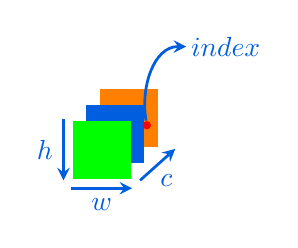
\begin{tikzpicture}
\coordinate (origin) at (0, 0);
\kernel{orange}{x}{(origin)};
\kernelPos{arrBlue}{x1}{left}{x}{(.6, -.2)};
\kernelPos{green}{x2}{left}{x1}{(.6, -.2)};
\tarrowNode{([shift={(-.1, 0)}]x2.north west)}{([shift={(-.1, 0)}]x2.south west)}{left}{$h$};
\tarrowNode{([shift={(0, -.1)}]x2.south west)}{([shift={(0, -.1)}]x2.south east)}{below}{$w$};
\tarrowNode{([shift={(.1, 0)}]x2.south east)}{([shift={(.2, 0)}]x.south east)}{right,shift={(-.1, -.2)}}{$c$};
\node[fill=red, circle, minimum size=.3em, inner sep=0pt] (point)at ([shift={(-.16, .3)}]x.south east) {};
\draw[arrStyle] (point) edge[out=100, in=180] ([shift={(.5, 1)}]point);
\node[\arrcolor](index) at ([shift={(1, 1)}]point) {$index$};
\end{tikzpicture}
\end{document}